\section{eo\-Init\-Generator$<$ EOT $>$ Class Template Reference}
\label{classeo_init_generator}\index{eoInitGenerator@{eoInitGenerator}}
turning an {\bf eo\-Init}{\rm (p.\,\pageref{classeo_init})} into a generator probably we should only use genrators - and suppress {\bf eo\-Init}{\rm (p.\,\pageref{classeo_init})} ??? MS - July 2001  


{\tt \#include $<$eo\-Init.h$>$}

Inheritance diagram for eo\-Init\-Generator$<$ EOT $>$::\begin{figure}[H]
\begin{center}
\leavevmode
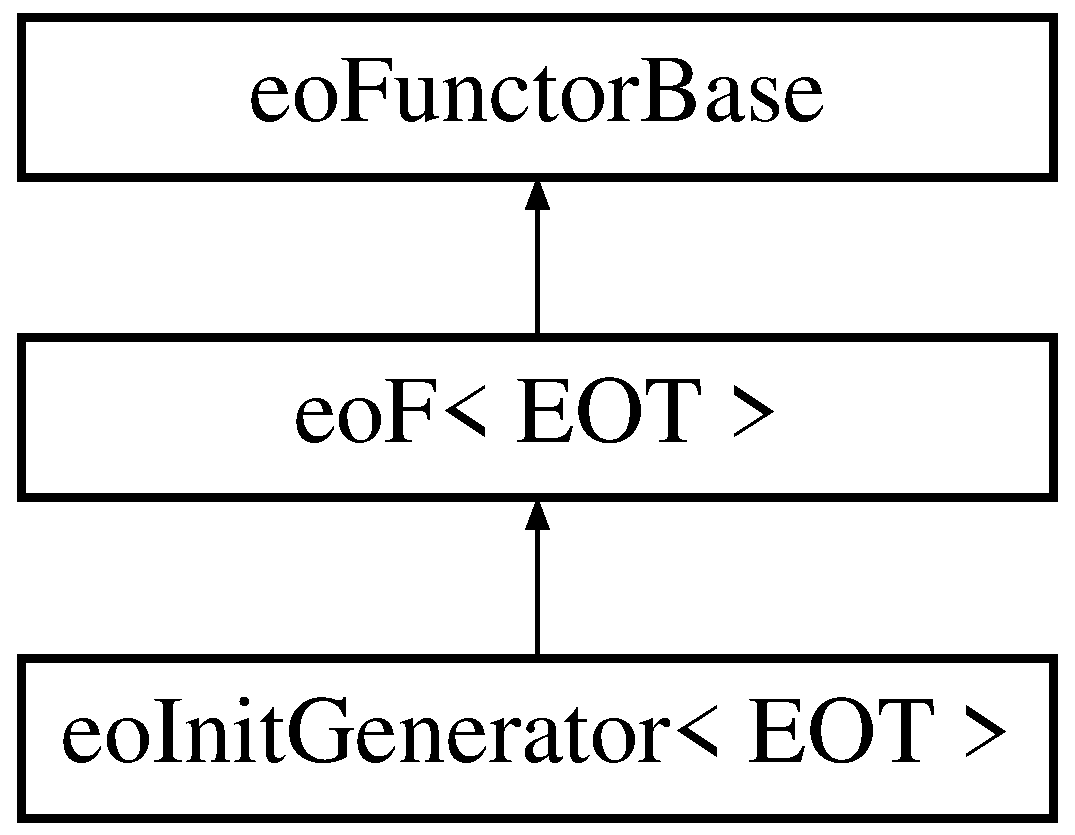
\includegraphics[height=3cm]{classeo_init_generator}
\end{center}
\end{figure}
\subsection*{Public Member Functions}
\begin{CompactItemize}
\item 
{\bf eo\-Init\-Generator} ({\bf eo\-Init}$<$ {\bf EOT} $>$ \&\_\-init)\label{classeo_init_generator_a0}

\begin{CompactList}\small\item\em Ctor from a plain {\bf eo\-Init}{\rm (p.\,\pageref{classeo_init})}. \item\end{CompactList}\item 
virtual {\bf EOT} {\bf operator()} ()\label{classeo_init_generator_a1}

\begin{CompactList}\small\item\em The pure virtual function that needs to be implemented by the subclass. \item\end{CompactList}\end{CompactItemize}
\subsection*{Private Attributes}
\begin{CompactItemize}
\item 
{\bf eo\-Init}$<$ {\bf EOT} $>$ \& {\bf init}\label{classeo_init_generator_r0}

\end{CompactItemize}


\subsection{Detailed Description}
\subsubsection*{template$<$class EOT$>$ class eo\-Init\-Generator$<$ EOT $>$}

turning an {\bf eo\-Init}{\rm (p.\,\pageref{classeo_init})} into a generator probably we should only use genrators - and suppress {\bf eo\-Init}{\rm (p.\,\pageref{classeo_init})} ??? MS - July 2001 



Definition at line 60 of file eo\-Init.h.

The documentation for this class was generated from the following file:\begin{CompactItemize}
\item 
eo\-Init.h\end{CompactItemize}
